\documentclass{conceptests}  
\begin{document}

% See mechanics/paddle-ball for an example of how to do wrapped figs.

\tableofcontents

\pagebreak

\addcontentsline{toc}{section}{Newton's laws}

\begin{qu}[Jump off a cliff]\num
You step off a 10 meter cliff and fall into a deep ocean pool below.
As you fall, the force of gravity on you...

A. is constant.

B. increases as you speed up.

C. is what initially changes your state of motion, but then it stops once you
stop accelerating.

D. equals your final velocity.

\end{qu}

\begin{qu}
\wrap{5}{50mm}{mechanics/figs/spinning-earth}
\num{} The earth spins on its axis once every day. This is caused by...

\noindent A. the force of inertia.

\noindent B. the force created by its velocity.

\noindent C. the force of gravity.

\noindent D. none of the above

\end{qu}

\begin{qu}
\wrap{5}{50mm}{mechanics/figs/paddle-ball}
\num{} You hit the ball with the paddle,
and when the rubber band becomes taut, it makes the ball come back to you.
Consider these forces:

$F_p$, a force of the paddle on the ball

$F_r$, a force of the rubber band on the ball

\noindent A. Both act at point 1 in the motion, and both also at 2.

\noindent B. $F_p$ acts at 1, and $F_r$ at 2.

\noindent C. $F_p$ acts at 1, and both act at 2.

\noindent D. Neither force acts at 1 or 2.

\end{qu}


\addcontentsline{toc}{section}{Gravity}

\begin{qu}[A wrench on the moon]\num
An astronaut on the moon, wearing a spacesuit, holds a wrench at chest height
and then releases it. What does the wrench do?

A. It floats upward.

B. It floats, staying at about the same height.

C. It floats, but may also move horizontally.

D. It falls to the ground.

\credit{Roger Feeley}
\end{qu}

\begin{qu}[An elliptical orbit]
\num
The figure shows a communications satellite traveling counterclockwise in an elliptical orbit.

\includegraphics{mechanics/figs/gravity-elliptical-orbit}

At the time indicated, the direction of the earth's gravitational force on the satellite is
most nearly

A, B, C, or

D. There is no gravity in outer space.
\end{qu}

\begin{qu}[A communications satellite's force on the earth]\num
A communications satellite is in a circular orbit arount the earth.
The satellite's gravitational force on the earth\ldots

A. is zero.

B. is nonzero but much less than the earth's gravitational force on it.

C. has a strength equal to the earth's gravitational force on it.


\credit{Jack Dostal}
\end{qu}

\begin{qu}\num
The circular orbits of satellites 1 and 2 coincide. Satellite 2 has
twice the mass of satellite 1. Compare their accelerations.

\vspace{20mm}

\includegraphics{mechanics/figs/gravity-coinciding-orbits}

A. 1's acceleration is half as much.

B. 1's acceleration is the same as 2's.

C. 1's acceleration is twice as much as 2's.

D. It depends on the periods of their orbits.
\end{qu}

\begin{qu}[$g/4$]\num
At which point is the earth's gravitational field 1/4 as strong as at P?

\vspace{20mm}

\includegraphics{mechanics/figs/gravity-one-fourth-g}

\pagebreak
\end{qu}

\begin{qu}\num
The large planet has 9 times more mass than the small one.
At which location is the gravitational field zero?

\vspace{20mm}

\includegraphics{mechanics/figs/gravity-earth-moon-cancel}
\end{qu}

\begin{qu}\num
 A wedge has been cut out of the earth to let us see inside it.
Points 1, 2, 3, and 4 all lie along the same radial line. Point 1 is at the
earth's center, 3 at its surface, and 2 in the interior of the earth at the
midpoint between 1 and 3.

Rank the points by the strength of their gravitational fields, from weakest
to strongest.

\includegraphics{mechanics/figs/gravity-inside-outside}

A. 4, 3, 2, 1

B. 4, 2, 3, 1

C. 1, 4, 2, 3

D. 1, 2, 4, 3
\end{qu}


\addcontentsline{toc}{section}{Energy and momentum}

\begin{qu}\num The dolphin is initially moving underwater, staying just below the surface, but it then coasts to
a halt and spends some time thinking about dolphin stuff. Describe the energy transformation.

\includegraphics{mechanics/figs/dolphin-energy}

A. PE to heat

B. KE to PE and heat

C. KE and PE to heat

D. KE to heat
\end{qu}

\begin{qu}\num
 Some buses in Switzerland contain massive flywheels that store
kinetic energy when the bus goes downhill, then release it when it needs to
go up again. If the velocity of the spinning wheel could be doubled, its
mass could be cut by a factor of

A. $\sqrt{2}$.

B. 2.

C. 4.

D. It would still have to have the same mass.

\end{qu}

\begin{qu}\num
Joe is asleep in the library.
The flea gets bored and leaps off of his arm. The flea's mass is smaller than
Joe's by a factor of $10^8$. After the flea is in the air, compare Joe's speed to the flea's.

\includegraphics{mechanics/figs/flea}

A. Joe isn't moving, but the flea is.

B. Joe recoils at a speed $10^{-8}$ that of the flea.

C. Joe recoils at a speed $10^{-16}$ that of the flea.

D. The whole planet earth recoils at an unmeasurably small speed.
\end{qu}

\begin{qu}[Recoil from a jumping flea, part 2]\num
 We adopt the frame
of reference in which Joe is initially at rest.
After the flea jumps, describe the kinetic
energy of the recoiling planet earth.

\includegraphics{mechanics/figs/flea}

A. The earth's KE is zero.

B. The earth gains much more KE than the flea.

C. The earth's larger mass and smaller speed give it the same KE as the flea.

D. The earth gains much less KE than the flea.

E. Energy is conserved, so the earth loses an amount of KE the same as what the flea gains.

\credit{Eric Mazur}

\end{qu}


\addcontentsline{toc}{section}{DC circuits}

\begin{qu}\num
In figure A, a charged rod acts on a charged ball from a certain
distance. In B, two such rods act from twice the distance on the same ball.

\vspace{20mm}

\includegraphics{electromagnetism/figs/two-rods-double-distance}

\noindent The deflections $\theta_A$ and $\theta_B$ of the strings from the vertical are

A. equal

B. unequal, with $\theta_A < \theta_B$

C. unequal, with $\theta_A > \theta_B$

D. need more information

\end{qu}

\begin{qu}\num
Electrical fuses are discussed in the text, without an explicit circuit diagram.
They work by heating to the point where they melt, opening the circuit.
The schematic symbol for a fuse is \includegraphics{electromagnetism/figs/fuse-symbol}.
Logically, which of the following arrangements would protect the
lightbulb from being burned out?

\vspace{20mm}

\includegraphics{electromagnetism/figs/fuse-and-bulb}
\end{qu}

\begin{qu}[Defroster]\num
The rear window in many cars has an electrical defroster consisting
of a grid of thin silver-ceramic lines that are essentially painted onto the glass.
A fixed voltage difference of 12 V from the car's battery is applied across the
defroster, which acts as a resistor with a resistance of on the order of one ohm.

Suppose that as a certain car gets older, physical changes in the grid cause its
resistance to \emph{decrease}. The amount of heat generated

\vspace{20mm}

A. goes down.

B. stays the same.

C. goes up.

D. There is no way to tell without more data.
\end{qu}

\begin{qu}\num
The two circuits are different, but they're made out of identical
batteries and lightbulbs. How do the currents compare?

\vspace{20mm}

\includegraphics{electromagnetism/figs/parallel-not-fixed-current}

\vspace{20mm}

A. $I_2$ and $I_3$ are each about half as big as $I_1$.

B. $I_2$ and $I_3$ are each about the same as $I_1$.

C. $I_2$ and $I_3$ are each about twice as big as $I_1$.

D. There is no way to tell without more data.
\end{qu}


\addcontentsline{toc}{section}{Relativity}

\begin{qu}\num
Eddie has always been his grandmother's favorite grandchild, so he
gets invited with her on an interstellar cruise. After the ship has accelerated
to 30\%
of the speed of light, Eddie unbuckles his seatbelt, hops out of his acceleration
couch, and extracts a folding meter-stick from his suitcase. Using the meter-stick,
he measures the length of the cabin from front to back.

\vspace{20mm}

A. The cabin measures more meters than before the ship accelerated.

B. The cabin measures fewer meters than before.

C. The cabin measures the same.

D. The effect is too small to be observable, because the ship's speed is still small compared
to the speed of light.
\end{qu}


\addcontentsline{toc}{section}{Optics}

\begin{qu}[Bad ray diagrams]\num
Correct the mistakes.

\includegraphics{optics/figs/bad-ray-diagrams}
\end{qu}


\end{document}
